%
%  MAIN driver/organizer for slide presentation
%

\documentclass[aspectratio=169]{beamer}

%%
\makeatletter
\defbeameroption{show only notes}[]% 
{
\beamer@notestrue
\beamer@notesnormalsfalse
}
\makeatother

\setbeameroption{hide notes}

%%  ... include packages

% !TEX root = ../digraph-main.tex
% packages.tex

\usetheme{Madrid}
\usepackage{appendixnumberbeamer}
\usefonttheme[onlymath]{serif}

% \usepackage{pgfplots}
%\usepackage{chronosys}

% fix booktabs compatibility issue
%\usepackage{etex}
%\usepackage{animate}

% math
%\usepackage{sansmathaccent}
\usepackage{amsmath}
\usepackage{amssymb}
\usepackage{amsthm}                 % Theorems/definitions
%\usepackage{mathrsfs}
\usepackage{array}
\usepackage{mathtools}

% SI units
\usepackage[detect-all]{siunitx}

% graphics
\usepackage[compatibility=false,justification=raggedright,
            font=scriptsize,labelformat=empty,skip=0pt,
            singlelinecheck=true]{caption}
\usepackage[labelformat=empty,justification=raggedright]{subcaption}
% \usepackage{graphicx}

\usepackage{xparse,fp}
%\usepackage{datenumber,xparse,fp}
\usepackage{pgf}
\usepackage{tikz}
\usetikzlibrary{arrows.meta}
\usetikzlibrary{decorations.text}
\usetikzlibrary{automata, positioning}
\usetikzlibrary{backgrounds}
\usetikzlibrary{tikzmark}
\usetikzlibrary{calc}
\usepackage{adjustbox}

% tables
\usepackage{multirow}
\usepackage{booktabs}
%\usepackage{colortbl}
%\usepackage{diagbox}
%\usepackage{arydshln} % dash line in tables
%\usepackage{makecell}
\usepackage{scalerel}

% clever references
\usepackage{cleveref}

% fonts
%% \usepackage{sfmath}
\usepackage{textcomp}
%\usepackage[resetfonts]{cmap}
\usepackage[utf8]{inputenc}
% \usepackage{natbib}

% \usepackage[
% backend=biber, 
% citestyle=ieee,
% sorting=nyt,    
% doi=false,
% url=false,
% isbn=false,
% giveninits=true,
% maxbibnames=9999,
% hyperref]{biblatex}

\usepackage[T1]{fontenc}
\usepackage{amsmath}

%\usepackage{fancybox} 
%\usepackage{framed,color}

% algorithm listing
\usepackage[noend]{algorithm2e}

% lists
% \usepackage{paralist}
\usepackage{enumerate}


%\usepackage[export]{adjustbox}


% fix cref
\crefname{proposition}{Proposition}{Propositions}
\Crefname{proposition}{Proposition}{Propositions}

\usepackage{bm}


% !TEX root = ../digraph-main.tex
% customization.tex


\definecolor{applegreen}{rgb}{0.55, 0.71, 0.0}
\definecolor{dukeblue}{RGB}{0, 83, 155}
\definecolor{navyblue}{RGB}{1, 33, 105}

\setbeamercolor{frametitle}{bg=navyblue, fg=white}
% \setbeamertemplate{section in toc}[sections numbered]
% \setbeamertemplate{subsection in toc}[subsections numbered]
% \useoutertheme[subsection=false]{miniframes}
% \setbeamercolor{section in head/foot}{fg=white, bg=dukeblue}
% \setbeamerfont{section in head/foot}{series=\bfseries}

% \makeatletter
% \setbeamertemplate{frametitle}{%
%   \nointerlineskip%
%   \begin{beamercolorbox}[%
%       wd=\paperwidth,%
%       sep=0pt,%
%       leftskip=\metropolis@frametitle@padding,%
%       rightskip=\metropolis@frametitle@padding,%
%       ht=2.25ex,%%%%%% NEW !!!!!!!!!!!!!!!!!!!!!!!!!!!!!!!!!!!!!!!!
%       dp=1.1ex, %%%%%% NEW !!!!!!!!!!!!!!!!!!!!!!!!!!!!!!!!!!!!!!!!
%     ]{frametitle}%
%   \metropolis@frametitlestrut@start%
%   \insertframetitle%
%   \nolinebreak%
%   \metropolis@frametitlestrut@end%
%   \end{beamercolorbox}%
% }
% \makeatother

% get rid of navigation symbols
\setbeamertemplate{navigation symbols}{}

% remove shadow from title block
\setbeamertemplate{title page}[default][colsep=-4bp,rounded=true]

% use square-type bullets
\setbeamertemplate{itemize item}[circle]
\setbeamertemplate{itemize subitem}{--}
\setbeamertemplate{enumerate item}[circle]

% use circles for ToC items and correct the weird size issue with "Madrid" theme
\setbeamertemplate{sections/subsections in toc}[circle]
\setbeamerfont{section number projected}{size=\normalsize}

% figure captions: no "figure" prefix, small text, small figure-caption space
\captionsetup[figure]{labelformat=empty}
\captionsetup[table]{labelformat=empty}
\captionsetup[figure]{font=tiny,labelfont=tiny}
\captionsetup[subfigure]{font=tiny,labelfont=tiny}

% command for fixing inline TikZ nodes' vertical alignment
\newcommand{\tikzbasefix}{-\the\dimexpr\fontdimen22\textfont2\relax}

% define coloured clickable links
\hypersetup{%
  pdffitwindow=false,%
  pdfstartview={FitH},%
  % colorlinks,%
  pdfauthor={},%
  pdftitle={},%
  pagebackref=true,%
  citecolor=PaleGreen4,%
  filecolor=DarkOrchid4,%
  % linkcolor=OrangeRed4,%
  urlcolor=RoyalBlue4%
}

% define the includegraphics search path
\graphicspath{%
  {./figures/}%
}

% short-hand command for hyperlinked e-mails
\newcommand{\email}[1]{\href{mailto:#1}{\texttt{#1}}}

% customize TikZ matrix column separator character (to avoid Beamer
% conflict)
\tikzset{ampersand replacement=\&}

% redefine \boxed command to allow setting the border color
\newcommand{\highlight}[1]{\fcolorbox{complclr1}{white}{$\displaystyle #1$}}

% remove extra spacing around \left and \right delimiters
\let\leftorig\left
\let\rightorig\right
\renewcommand{\left}{\mathopen{}\mathclose\bgroup\leftorig}
\renewcommand{\right}{\aftergroup\egroup\rightorig}

% increase vertical spacing between table rows
\renewcommand{\arraystretch}{1.2}

% modified bullet-point for highlighting
\newcommand{\bulletemph}{$\large\boldsymbol{\star}$}

% superscript comma for footnote references
\newcommand{\footcomma}{\textsuperscript{,}}

% command to output names under images
\newcommand{\imentry}[3][1.25cm]{%
  \vbox{\halign{\hfil##\hfil\cr%
      \includegraphics[height=#1]{#2}\cr#3\cr}}}

% pictures goes with authors
\newcommand{\theauthor}[2]{\vbox{\halign{\hfil##\hfil\cr
  \includegraphics[width=0.125\textwidth]{#1}\cr#2\cr}}}

\newcommand{\theauthornopic}[1]{\vbox{\halign{\hfil##\hfil\cr
  \cr#1\cr}}}

\DeclareCaptionFont{tiny}{\tiny}

\newcommand{\backupbegin}{
   \newcounter{finalframe}
   \setcounter{finalframe}{\value{framenumber}}
}
\newcommand{\backupend}{
   \setcounter{framenumber}{\value{finalframe}}
}

\setbeamerfont{footnote}{size=\tiny}

% timeline option
\newlength\yearposx

% fix bug in beamer
% [https://tex.stackexchange.com/a/426090]
\makeatletter
\let\@@magyar@captionfix\relax
\makeatother

% alternative footnote by Tiancheng Liu
\newcommand\alternativefootnote[1]{%
 \tikz[remember picture,overlay]
 \draw (current page.south west) +(1in + \oddsidemargin,1em)
 node[anchor=south west,inner sep=0pt]{\parbox{\textwidth}{%
     \rlap{\rule{10em}{0.4pt}}\raggedright\tiny#1}};}


\def\signed #1{{\leavevmode\unskip\nobreak\hfil\penalty50\hskip1em
    \hbox{}\nobreak\hfill #1%
    \parfillskip=0pt \finalhyphendemerits=0 \endgraf}}

\newsavebox\mybox
\newenvironment{aquote}[1]
{\savebox\mybox{#1}\begin{quote}\hspace*{-.7ex}}
  {\unskip\vspace*{1mm}\signed{\usebox\mybox}\end{quote}}


% define new table columns for fixed-width center columns
% 
% [https://tex.stackexchange.com/a/12712]
\newcolumntype{C}[1]{>{\centering\let\newline\\\arraybackslash\hspace{0pt}}m{#1}}

% change how sections and subsection are highlight in TOC
\setbeamertemplate{section in toc}{
  \textbf{\inserttocsectionnumber.~\inserttocsection}}
\setbeamertemplate{section in toc shaded}{
  \inserttocsectionnumber.~\inserttocsection}

\setbeamertemplate{subsection in toc}{
  \hspace{1.2em}{\rule[0.3ex]{3pt}{3pt}}~\textbf{\inserttocsubsection}\par}
\setbeamertemplate{subsection in toc shaded}{
  \hspace{1.2em}{\rule[0.3ex]{3pt}{3pt}}~\inserttocsubsection\par}

% clever ref
\crefname{equation}{}{}
\Crefname{equation}{}{}

% extra rule for adding image with raggedright centered caption
\newcommand{\lcaption}[2]{ %
  % 
  \captionsetup{justification=raggedright}
  % 
  \begin{minipage}{#1}
    \caption{ %
      #2
    }
  \end{minipage}
}

\DeclareSIUnit{\nothing}{\relax}

\newcommand*{\textcal}[1]{%
  % family qzc: Font TeX Gyre Chorus (package tgchorus)
  % family pzc: Font Zapf Chancery (package chancery)
  \textbf{\textit{\fontfamily{qzc}\selectfont#1}}% 
}

\DeclareMathAlphabet{\zcal}{\encodingdefault}{sqzc}{m}{it}


\addtobeamertemplate{frametitle}{}{\vspace*{-0.5em}}


\newcommand{\gls}{G$\ell$S}

\newcommand{\conf}{\Omega}

\newcommand{\ha}{h_{\rm a}}
\newcommand{\hr}{h_{\rm r}}
\newcommand{\dm}{{{\em d.m.}}}

\newcommand{\bluered}{br}

\setbeamercolor{block body}{bg=dukeblue!30}
\setbeamercolor{block title}{bg=dukeblue,fg=black!2}


% theorem and collorary
\setbeamertemplate{theorems}[numbered] 

\makeatletter
\g@addto@macro\normalsize{%
    \setlength\abovedisplayskip{2pt}
}
\g@addto@macro\normalsize{%
    \setlength\belowdisplayskip{2pt}
}

\newcommand{\smsp}{\mspace{2mu}}  % slightly smaller space than \,
\DeclareMathOperator*{\argmax}{arg \smsp max}
\DeclareMathOperator*{\argmin}{arg \smsp min}

\newtheorem{proposition}{Proposition}


\def\arrowtext#1#2{\hbox to#1{\arrowtextA\ #2 \arrowtextA\kern2pt\llap{$\succ$}}}
\def\arrowtextA{\leaders\vrule height2.7pt depth-2.3pt\hfil}

\newcommand{\tikzvrule}[1]{
  \draw   ([yshift=-0.8cm,xshift=#1]current page.north west)
       -- ([xshift=#1]current page.south west)
}

\newcommand{\tikzvsubrule}[3]{
  \draw   ([yshift=-0.8cm+#2,xshift=#1]current page.north west)
       -- ([yshift=-0.8cm+#3,xshift=#1]current page.north west)
}

\newcommand{\tikzhrule}[1]{
  \draw   ([yshift=-0.8cm+#1]current page.north west)
       -- ([yshift=-0.8cm+#1]current page.north east)
}

\newcommand{\tikzhsubrule}[3]{
  \draw   ([yshift=-0.8cm+#1,xshift=#2]current page.north west)
       -- ([yshift=-0.8cm+#1,xshift=#3]current page.north east)
}


% footnote size & enable footnotes
% \renewcommand{\footnotesize}{\fontsize{5pt}{8pt}\selectfont}
% \let\oldfootnote\footnote
% \renewcommand\footnote[1][]{\oldfootnote[frame,#1]}

\renewcommand*{\bibfont}{\tiny}

% \AtEveryCitekey{
% %   \clearfield{location}
%   \clearfield{title}
%   \clearfield{number}
%   \clearfield{volume}
% %   \clearfield{publisher}
% }

\renewbibmacro*{cite}{%
  \iffieldundef{shorthand}
    {\ifthenelse{\ifnameundef{labelname}\OR\iffieldundef{labelyear}}
       {\usebibmacro{cite:label}%
        \setunit{\printdelim{nonameyeardelim}}}
       {\printnames{labelname}%
        \setunit{\printdelim{nameyeardelim}}}%
     \usebibmacro{cite:labeldate+extradate}%
     \setunit{\addcomma\space}%
     \usebibmacro{journal}}
   {\usebibmacro{cite:shorthand}}}

\setbeamertemplate{bibliography item}{}

%\makeatletter
%\newcommand{\xleftrightarrow}[2][]{\ext@arrow 3359\leftrightarrowfill@{#1}{#2}}
%\makeatother


% !TEX root = ../digraph-main.tex
% graphics.tex


% ---------- colors ---------- %

% color palette
\definecolor{baseclr}{HTML}{27408B}
\definecolor{myclr}{HTML}{000000}
\definecolor{complclr}{HTML}{CE9927}

% 2 complementary color sets
\definecolor{myblue}{HTML}{27408B}
\definecolor{myorange}{HTML}{CE9927}
\definecolor{myred}{HTML}{A92066}
\definecolor{mygreen}{HTML}{86BF24}

% alternative green-red combination
\definecolor{otherred}{HTML}{AA3939}
\definecolor{othergreen}{HTML}{2E882E}

% beamer colors
\setbeamercolor{normal text}{fg=baseclr}
\setbeamercolor{section in toc}{fg=baseclr}
\setbeamercolor{subsection in toc}{fg=baseclr}

% shade colors & listings

\definecolor{lightgray}{gray}{0.95} 
\definecolor{shadecolor}{rgb}{0.95,0.95,0.85}    % weights by xiaobai 

\sloppy



% !TEX root = ../digraph-main.tex
% extras.tex


\usetheme{Madrid}
\setbeamertemplate{caption}[numbered]
\setbeamertemplate{caption label separator}{: }
\setbeamercolor{caption name}{fg=normal text.fg}
\usepackage{lmodern}
\usepackage{amssymb,amsmath}
\usepackage{ifxetex,ifluatex}
\usepackage{fixltx2e} % provides \textsubscript
\ifnum 0\ifxetex 1\fi\ifluatex 1\fi=0 % if pdftex
  \usepackage[T1]{fontenc}
  \usepackage[utf8]{inputenc}
\else % if luatex or xelatex
  \ifxetex
    \usepackage{mathspec}
  \else
    \usepackage{fontspec}
  \fi
  \defaultfontfeatures{Mapping=tex-text,Scale=MatchLowercase}
  \newcommand{\euro}{€}
\fi
% use upquote if available, for straight quotes in verbatim environments
\IfFileExists{upquote.sty}{\usepackage{upquote}}{}
% use microtype if available
\IfFileExists{microtype.sty}{%
\usepackage{microtype}
\UseMicrotypeSet[protrusion]{basicmath} % disable protrusion for tt fonts
}{}
\usepackage{listings}
\usepackage{graphicx,grffile}
\makeatletter
\def\maxwidth{\ifdim\Gin@nat@width>\linewidth\linewidth\else\Gin@nat@width\fi}
\def\maxheight{\ifdim\Gin@nat@height>\textheight0.8\textheight\else\Gin@nat@height\fi}
\makeatother
% Scale images if necessary, so that they will not overflow the page
% margins by default, and it is still possible to overwrite the defaults
% using explicit options in \includegraphics[width, height, ...]{}
\setkeys{Gin}{width=\maxwidth,height=\maxheight,keepaspectratio}

% Comment these out if you don't want a slide with just the
% part/section/subsection/subsubsection title:
% \AtBeginPart{
%   \let\insertpartnumber\relax
%   \let\partname\relax
%   \frame{\partpage}
% }
%\AtBeginSection{
%  \let\insertsectionnumber\relax
%  \let\sectionname\relax
%  \frame{\sectionpage}
%}
%\AtBeginSubsection{
%  \let\insertsubsectionnumber\relax
%  \let\subsectionname\relax
%  \frame{\subsectionpage}
%}

% show plan before each section
% \AtBeginSection[]
% {
%   \begin{frame}[noframenumbering,plain]
%     % \frametitle{Outline}
%     \tableofcontents[currentsection,
%         currentsubsection,
%         subsectionstyle=show/show/hide]
%   \end{frame}
% }

\setlength{\emergencystretch}{3em}  % prevent overfull lines
\providecommand{\tightlist}{%
  \setlength{\itemsep}{0pt}\setlength{\parskip}{0pt}}
\setcounter{secnumdepth}{0}

%% ============ set up the title slide and footer information

% title.tex


\title%
[Perfusion Model (Convolution and ODE)]%                                %%  short version for footer
{Group Meeting: Perfusion Model (Convolution and ODE)}%             %%  long version

% \subtitle                                                                      %% used for location and time of presentation
% {\vspace*{0.5em}\footnotesize
%     \\
%   Oct.   2021
% }

% -------------------- AUTHOR LIST ( & short info in FOOTER )

\author%
[Juntang Wang]%                                    %% including photos and short info for FOOTER
{%
  % \theauthornopic{Dimitris Floros\footnotemark[1]}  %% without picture
  \theauthor{authors/JW}{Juntang Wang\footnotemark[1]}
  \theauthor{authors/YG}{Yike Guo\footnotemark[1]}
  \theauthor{authors/SX}{Shixin Xu\footnotemark[1]}
  % \theauthor{authors/XS}{Xiaobai Sun\footnotemark[1]}
  % \theauthor{authors/NP}{Nikos Pitsianis\footnotemark[3]}
  % \theauthor{authors/DF}{Dimitris Floros\footnotemark[1]}
  % \theauthor{authors/TL}{Tiancheng Liu\footnotemark[4]}
}

\institute%
[Duke Kunshan]% % short for FOOTER info
{%

  % \inst{1}
  % Duke University, NC, USA%,
  
  \inst{1}
  Duke Kunshan University, China%,

  % \inst{3}
  % Aristotle University of Thessaloniki, Greece%.

  % \inst{4}
  % Meta, PA, USA%.
}

\date%
[\today]%
{\today}


% ========== bibliography
\bibliography{MATH.bib}

\begin{document}


\frame{\titlepage}                     % the very first slide frame 

\begin{frame}[noframenumbering,plain]
  \frametitle{Outline}
  \tableofcontents
\end{frame}

%%  ---------- Outline 
% \part{Part I}



%% ----------- Problem description 

\section{Backgrounds}
\subsection{Problem Description}
% problem-description.tex
%
% Drafted by Juntang on August 20, 2024
%

\begin{frame}
  \frametitle{Problem Description}
    Goal: to obtain quantitative \textbf{perfusion indices} from pwiMRI images
    \begin{itemize}
        \item \textbf{CBF}: Cerebral Blood Flow. The rate at which blood is delivered. $Q [mL/100g]$
        \item \textbf{CBV}: Cerebral Blood Volume. The total volume of blood present. $V[mL/100g]$
        \item \textbf{MTT}: Mean Transit Time. The average duration that blood spends transiting. $MTT[s]$
        \item $\mathbf{T_{max}}$: Time to Maximum of the Residue Function. The time required for the residue function of a tracer to reach its peak, indicative of cerebral perfusion efficiency. $T_{max}[s]$
    \end{itemize}

\end{frame}

%%% Local Variables:
%%% mode: latex
%%% TeX-master: "../topic-slide-main"
%%% End:
\subsection{Assumptions}
% assumptions.tex
%
% Drafted by Juntang on August 20, 2024
%

\begin{frame}
  \frametitle{Assumptions}
    \cite{zierlerTheoreticalBasisIndicatorDilution1962}
    \begin{itemize}
        \item Single inflow and a single outflow orifice
        \item Recirculation does not occur
        \item Flow and volume be constant
        \item The system must exhibit stationarity (constant distribution of transit times)
        \item Distribution of transit times of indicator particles be identical with the distribution of transit times of the native fluid

    \end{itemize}

\end{frame}

%%% Local Variables:
%%% mode: latex
%%% TeX-master: "../topic-slide-main"
%%% End:

\subsection{Gamma Variate Function}
% gamma-variate.tex
%
% Drafted by Juntang on August 20, 2024
% Adjusted by Juntang on August 22, 2024

\begin{frame}
  \frametitle{Gamma Variate Function}
    \cite{thompsonIndicatorTransitTime1964}
    \begin{columns}
    %% double-column layout 
    \begin{column}{0.45\textwidth}                 %% Left Column 
    {\small
    \begin{itemize}
        \item GVF \& Adj. Sheppard's model:
    \end{itemize}
    \begin{equation}
    C(t) = k(t - AT)^{\alpha} e^{-\frac{(t - AT)}{\sigma}}
    \end{equation}
    \begin{equation}
    C(t) = \frac{A (t - AT)^{\alpha}}{\Gamma(1 + \alpha) \sigma^{1+\alpha}} e^{-\frac{(t - AT)}{\sigma}}
    \end{equation}

    $\begin{aligned}
        t &= \text{time after injection} \\
        C(t) &= \text{indicator concentration at time, } t \\
        k &= \text{constant scale factor} \\
        AT &= \text{appearance time} \\
        \alpha, \sigma &= \text{arbitrary parameters, } 1/\sigma = Q/V \\
        A &= \text{total area under the curve, } I/Q
    \end{aligned}$
    }
    \end{column}
    
    \hspace*{4em}                                                          %%  make space between columns 
    
    \begin{column}{0.42\textwidth}                                %% Right Column 
        Indicator transit time has been shown to exhibit the mathematical properties of a general class of random variables, known as "gamma variates." Curve-fitting techniques were employed to show that the arterial indicator curves are equivalent to frequency distribution functions for this class of variables.
    \end{column}
    %
    \end{columns}   %% End of multiple columns 
    % 

\end{frame}

%%% Local Variables:
%%% mode: latex
%%% TeX-master: "../topic-slide-main"
%%% End:
\subsection{Gamma Variate Function More}
% gamma-variate.tex
%
% Drafted by Juntang on Sep 23, 2024
% 

\begin{frame}
  \frametitle{Gamma Variate Function - More}

    \begin{columns}
    %% double-column layout 
    \begin{column}{0.45\textwidth}                 %% Left Column 
    {\footnotesize
    \cite{davenportDerivationGammaVariateRelationship1983}

    \begin{itemize}
        \item ODE from Indicator-Dilution Theory \newline (\cite{zierlerTheoreticalBasisIndicatorDilution1962}):
    \end{itemize}
    \begin{equation}
    \frac{dC_{i}(t)}{dt} = \frac{Q}{V} (C_{i-1}(t) - C_{i}(t))
    \end{equation}
    {\tiny
    where $i$ is the indice of the chamber
    
    \(
    C_{1}(t) = C_{0}e^{-t/\sigma} 

    C_{2}(t) = C_{0}\frac{t}{\sigma}e^{-t/\sigma} 

    C_{3}(t) = \frac{C_{0}}{2}(\frac{t}{\sigma})^{2}e^{-t/\sigma}
    \)}
    \vspace{-8pt}
    \begin{equation}
    \Leftrightarrow C_{n}(t) = \frac{C}{(n-1)!}(\frac{t}{\sigma})^{n-1}e^{-t/\sigma}
    \end{equation}
    {\tiny
    let $\alpha = n - 1, \; C_0 = \frac{\Gamma(\alpha)}{\sigma\Gamma(\alpha+1)} \Leftrightarrow \int^{\infty}_{0}C(t)dt = 0 $
    }
    \vspace{-8pt}
    \begin{equation}
    \Leftrightarrow C(\alpha, \sigma, t) = \frac{t^\alpha}{\Gamma(\alpha+1)\sigma^{\alpha+1}}e^{-t/\sigma}
    \end{equation}

    
    }
    \end{column}
    
    \hspace*{4em}                                                          %%  make space between columns 
    
    \begin{column}{0.5\textwidth}                                %% Right Column 
    {\tiny
    \begin{block}{\textwidth}
        \tiny
        \cite{sheppardMathematicalConsiderationsIndicator1954}
        \begin{itemize}
            \item Stochasic model where tracer follow $1d$ random walk; Poisson distribution:
        \end{itemize}
        \begin{equation}
            C(t) = \frac{t^{n-1}}{(n-1)!(1/n)^{n}}e^{-nt}
        \end{equation}
        reduced to a GVF by substituting
    
        \(
        \alpha = n - 1
    
        \sigma = 1 / n
        \)
        \begin{itemize}
            \item CON: not $\sigma > 1$ (\cite{thompsonIndicatorTransitTime1964})
        \end{itemize}
    \end{block}

    \begin{itemize}
        \item PRO: deterministic, theoretical $\rightarrow$ physiologic
    \end{itemize}
    {\tiny
    \(
    L[f(s)] = \int_0^\infty e^{-st} f(t) dt
    \)
    and
    \(
    f*C = \int_0^t f(t-\tau) C(\alpha, \beta, \tau) d\tau
    \)
    \(
    f(t) = \int_{C-i\infty}^{C+i\infty} L[f(s)] ds
    \)
    where C is selected s.t. the path of integration is to the right of all singularities of L[f] within the complex plane.

    \(
    f(t) = L^{-1}\left(\frac{L[f*C]}{L[C]}\right)
    \)
    by the convolution theorem
    \(
    L[f*g] = L[f]L[g]
    \)
    }
    
    ...
    
    For recirculations:
    \begin{equation}
    D(t) = C(\alpha, \beta, t) + C(2\alpha+1, \beta, t-T) + C(3\alpha+2, \beta, t-2T) + \dots
    \end{equation}
    
    }
    \end{column}
    %
    \end{columns}   %% End of multiple columns 
    % 

\end{frame}



%%% Local Variables:
%%% mode: latex
%%% TeX-master: "../topic-slide-main"
%%% End:
\subsection{State of the Art (I)}
% state-of-the-art_patent.tex
%
% Drafted by Juntang on August 21, 2024
% ReDragted by Juntang on August 22, 2024

\begin{frame}
  \frametitle{State of the Art (I)}
  \cite{Dt_patent_wo2005104936a12005}
    \begin{columns}
    %% double-column layout 
    \begin{column}{0.45\textwidth}                 %% Left Column
    {\small
    \begin{enumerate}
        \item $C_{AIF} \rightarrow C_{in}$, assuming $\alpha_1 = 0$:
        \begin{equation}
            C_{in}(t) = \left( C_{AIF} * R_{1}^{[P]} \right)(t)
        \end{equation}
        \begin{equation}
            R_{1}^{[P]}(t) = \left\{
            \begin{array}{ll}
            \frac{1}{\sigma_1} e^{-\frac{t - AT_1}{\sigma_1}}, & \text{if } t \geq AT_1 \\
            0, & \text{otherwise}
            \end{array}\right.
        \end{equation}
        %
        \item $C_{in} \rightarrow C_{tissue}$, assuming $AT_2 = 0$:
        \begin{equation}
        C_{tissue}(t) = \frac{Q}{k_H}\left( C_{in} * R_{2}^{[P]} \right)(t)
        \end{equation}
        \begin{equation}
            R_{2}^{[P]}(t) = 1 - \int_0^t \frac{\tau^{\alpha_2}}{\Gamma(1 + \alpha_2) \sigma_2^{1+\alpha_2}} e^{-\frac{\tau}{\sigma_2}} d\tau 
        \end{equation}
    \end{enumerate}
    }
    \end{column}
    
    \hspace*{4em}                                                          %%  make space between columns 
    
    \begin{column}{0.42\textwidth}                 %% Right Column 
        \begin{figure}
            \centering
            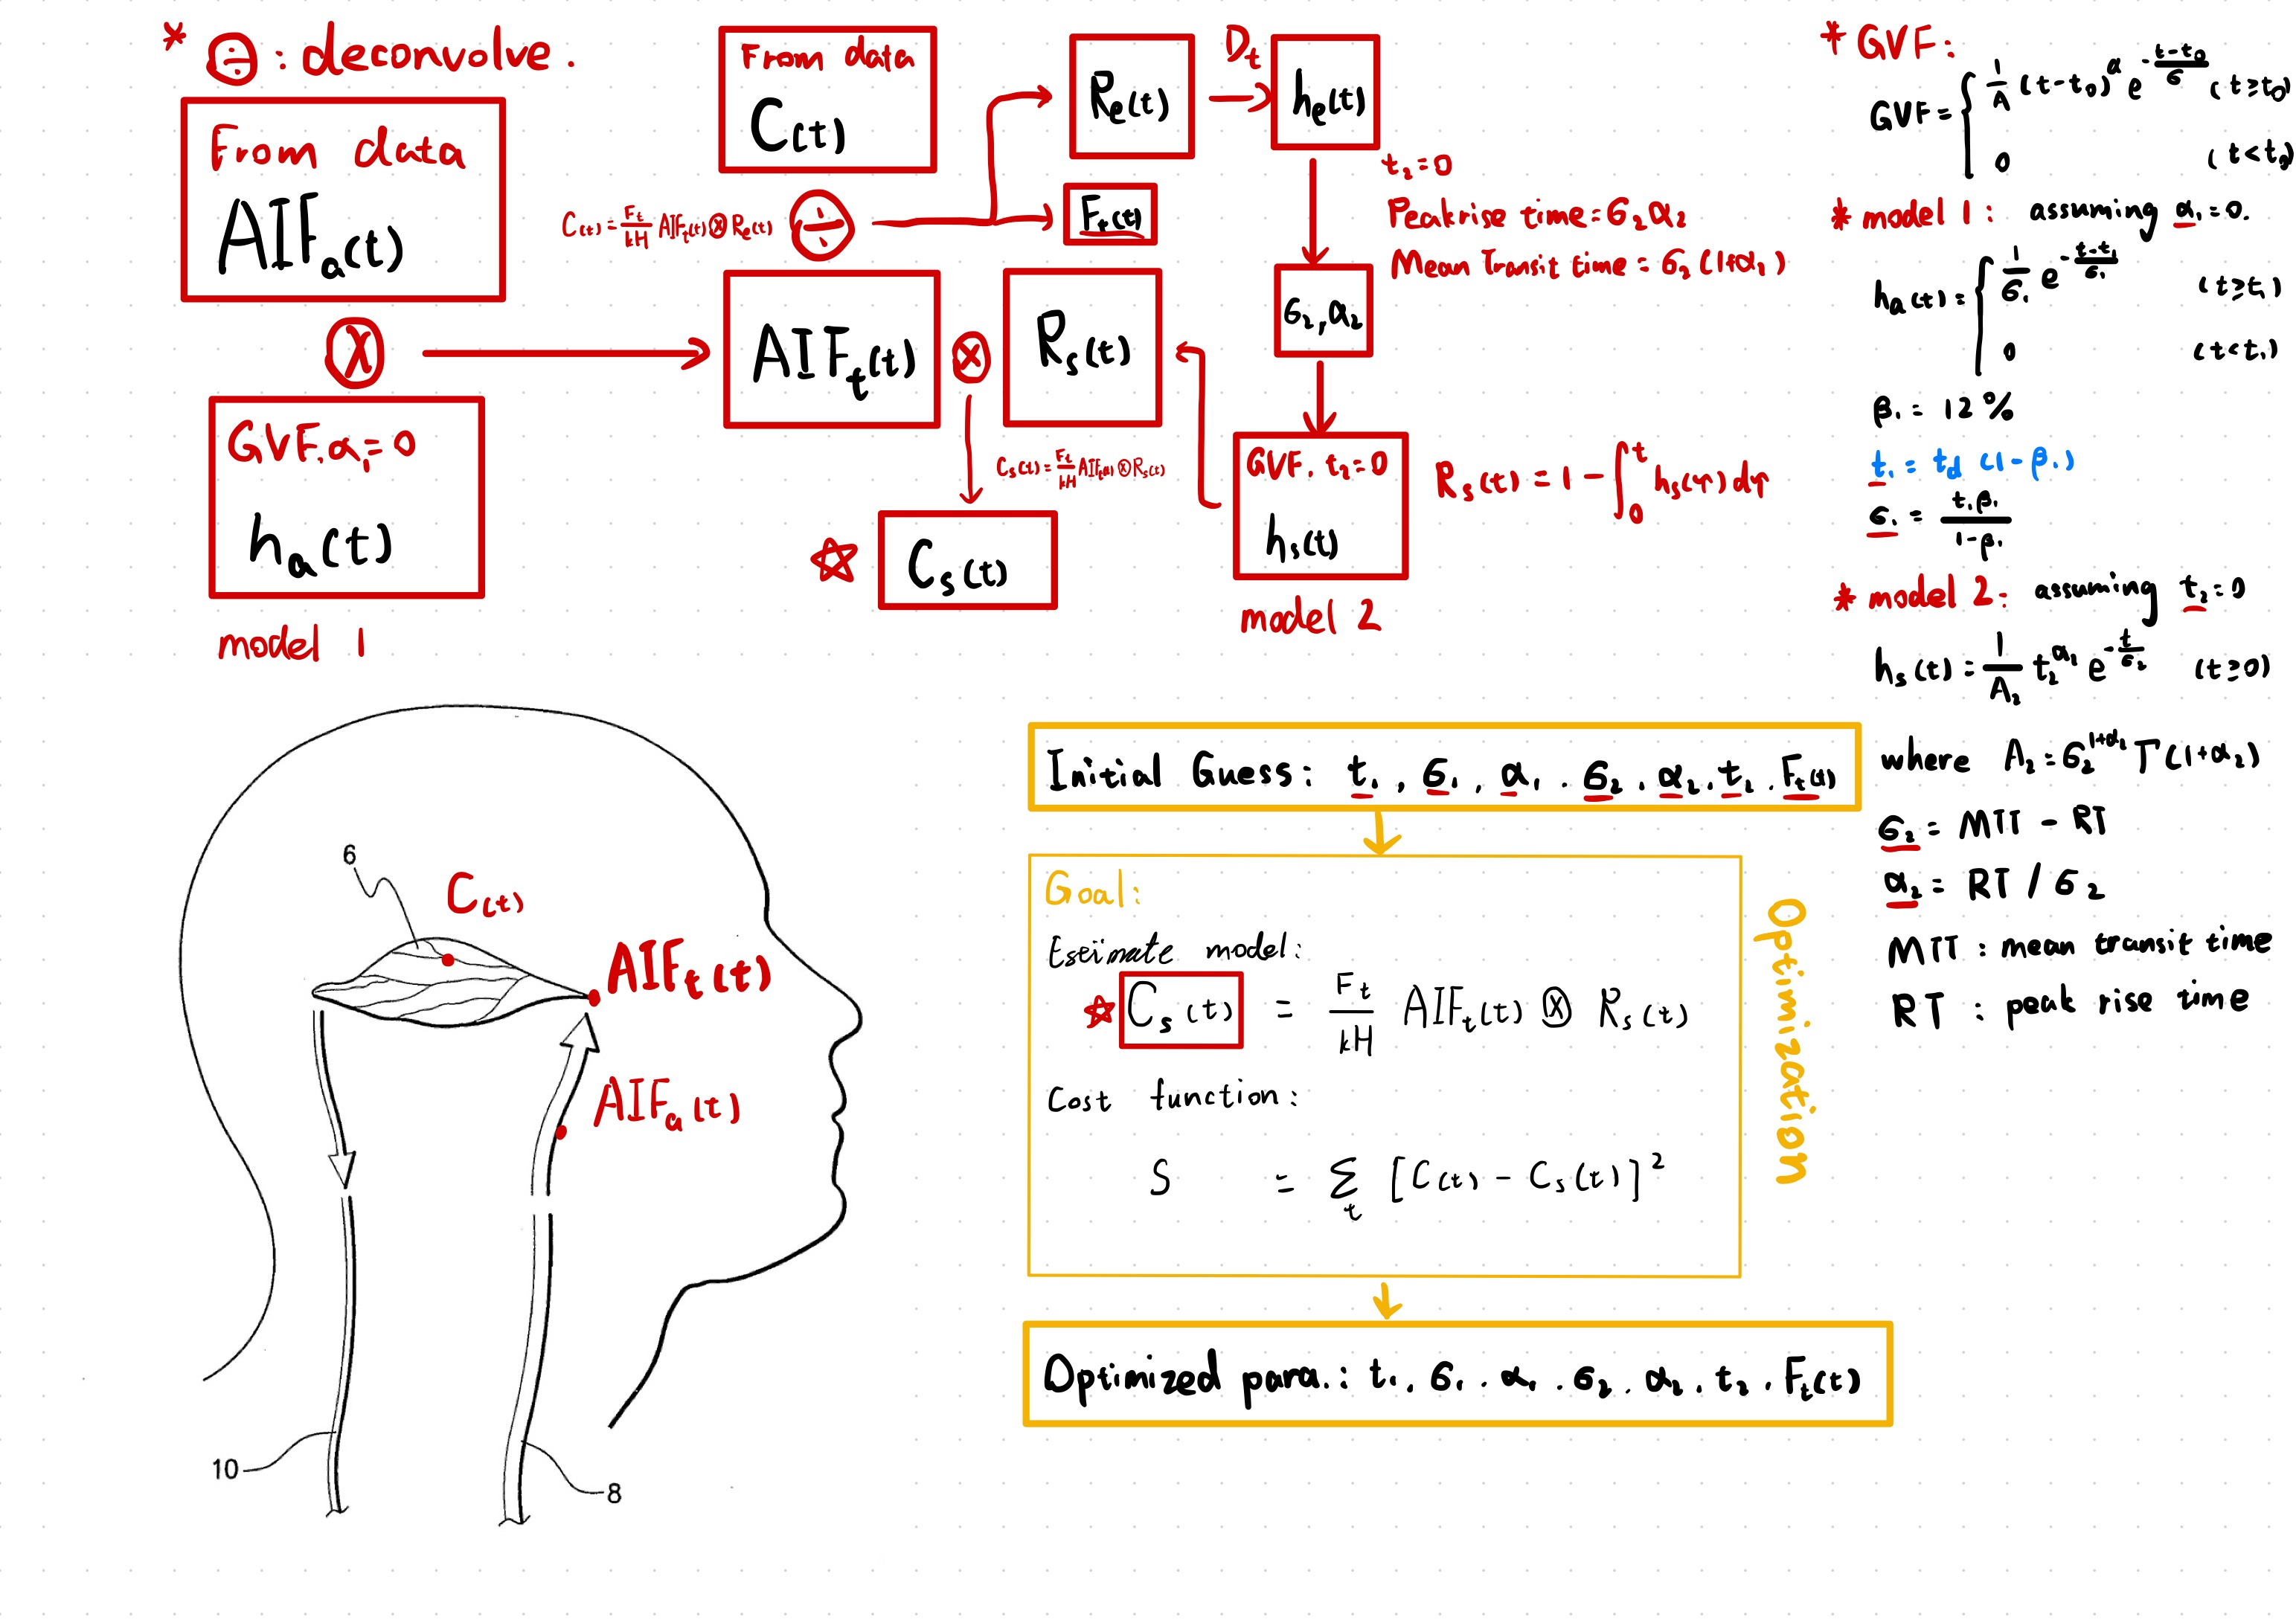
\includegraphics[width=\linewidth]{figures/intro-patent.jpg}
            \caption{Flowchart summarizing the methodology of \cite{Dt_patent_wo2005104936a12005}}
            \label{fig:patent}
        \end{figure}
    \end{column}
    %
    \end{columns}   %% End of multiple columns 
    % 

\end{frame}

%%% Local Variables:
%%% mode: latex
%%% TeX-master: "../topic-slide-main"
%%% End:
\subsection{State of the Art (II)}
% state-of-the-art_straka.tex
%
% Drafted by Juntang on August 22, 2024
% 

\begin{frame}
  \frametitle{State of the Art (II)}
  \cite{strakaRealTimeDiffusion2010}
    \begin{columns}
    %% double-column layout 
    \begin{column}{0.45\textwidth}                 %% Left Column 
    {\small
    \begin{enumerate}
        \item $C_{AIF} \rightarrow (C_{in}) \rightarrow C_{tissue}$:
        \begin{equation}
            C_{tissue}(t) = \left( C_{AIF} * R_{1\&2}^{[S]} \right)(t)
        \end{equation}
        \begin{equation}
            R_{1\&2}^{[S]}(t) = \frac{1}{TR}FT^{-1}\{g(f)\frac{c_t(f)}{c_a(f)}\}
        \end{equation}
        
        \item[] where:
        $\begin{aligned}
            c_t(f) &= FT\{C_{tissue}'(t)\} \\
            c_a(f) &= FT\{C_{AIF}'(t)\} \\
            g(f) &= {\left\{
            \begin{array}{lll}
            \frac{c_a(f)^2-N^2}{c_a(f)^2} & \text{if } c_a(f)>N, f\neq0 \\
            1 & \text{if } f=0 \\
            0 & \text{otherwise}
            \end{array}
            \right.}
        \end{aligned}$  
         {\tiny $TR$ is sampling rate, $FT{}$ denotes Fourier Transform, and $'$ denotes signal zero padded.}
    \end{enumerate}
    }
    \end{column}
    
    \hspace*{4em}                                                          %%  make space between columns 
    
    \begin{column}{0.42\textwidth}                 %% Right Column 
        \begin{figure}
            \centering
            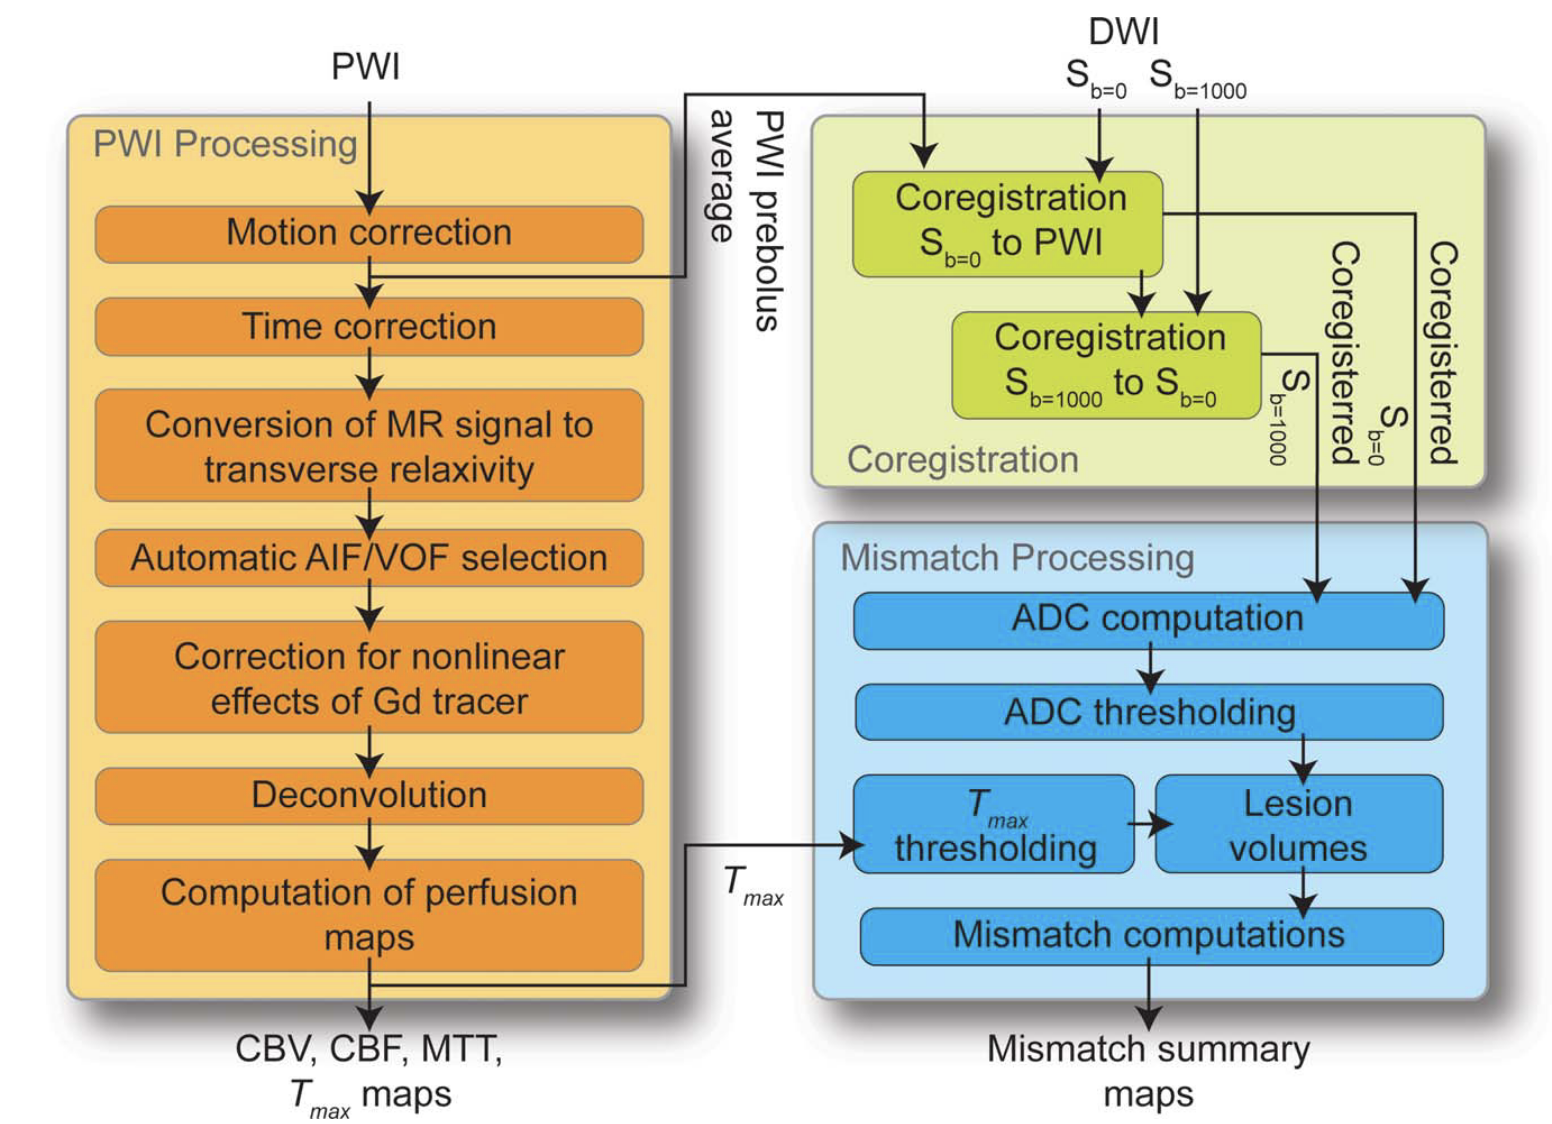
\includegraphics[width=\linewidth]{figures/intro-straka.png}
            \caption{Details of the RAPID pipeline used to calculate mismatch between DWI and PWI from \cite{strakaRealTimeDiffusion2010}.}
            \label{fig:straka}
        \end{figure}
    \end{column}
    %
    \end{columns}   %% End of multiple columns 
    % 

\end{frame}

%%% Local Variables:
%%% mode: latex
%%% TeX-master: "../topic-slide-main"
%%% End:



%% ----------- Method

\section{Method}
\subsection{Our Model}
% method-our-model.tex
%
% Drafted by Juntang on August 22, 2024
% Adj T on Sep 23, 24

\begin{frame}
  \frametitle{Our Model}
    \begin{columns}
        \column{0.68\textwidth}
        \begin{block}{}
        \begin{equation}
            \Leftrightarrow \sigma \frac{dC_{i}(t)}{dt} + C_{i}(t) = C_{i-1}(t-AT) u(t-AT)
        \end{equation}
        \begin{equation}  
            \begin{aligned}
                R(t) = C_n(t) &= {\left\{
                \begin{array}{ll}
                \frac{t^\alpha}{\Gamma(\alpha+1)\sigma^{\alpha+1}} e^{-\frac{t - AT_1}{\sigma_1}}, & \text{if } t \geq AT_1 \\
                0, & \text{otherwise}
                \end{array}
                \right.}
            \end{aligned}
        \end{equation}
        \vspace{-13pt}
        \begin{enumerate}
            \item $C_{AIF} \rightarrow C_{in}$:
            \begin{equation}
                C_{in}(t) = \frac{k_H}{\kappa} \left( C_{AIF} * R_{1}^{[P]} \right)(t)
            \end{equation}
            %
            \item $C_{in} \rightarrow C_{tissue}$:
            \begin{equation}
            C_{tissue}(t) = \left( C_{in} * R_{2} \right)(t)
            \end{equation}

            \item[] where:
            
            $\begin{aligned}
                k_H &= \left(\frac{1 - H_{LV}}{1 - H_{SV}}\right) \\
                \kappa &= \int_0^T C_a(\tau) d\tau / \int_0^T C_v(\tau) d\tau
            \end{aligned}$    
            
        \end{enumerate}
        \end{block}

        \hspace*{4em}  

        \column{0.23\textwidth}
        \begin{figure}[h]
            \centering
            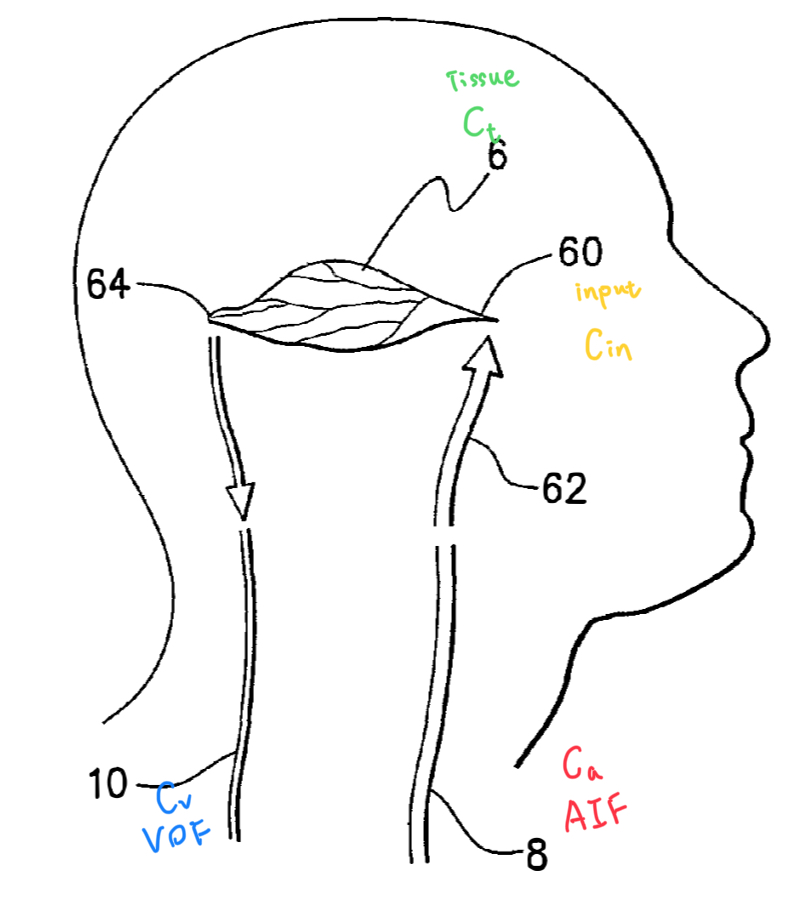
\includegraphics[width=\textwidth]{figures/method-our.jpeg}
            \caption{Diagram of the system illustrating the different concentrations involved in the model. \(C_a\) (red) represents the arterial input function (AIF), \(C_{in}\) (yellow, imaginary) represents the entrance concentration, \(C_t\) (green) represents the tissue concentration, and \(C_v\) (blue) represents the venous output function (VOF). }
            \label{fig:solution_plot}
        \end{figure}
        
        
    \end{columns}
   

\end{frame}

%%% Local Variables:
%%% mode: latex
%%% TeX-master: "../topic-slide-main"
%%% End:
\subsection{Comparison of Kernels}
% method-comparision.tex
%
% Drafted by Juntang on August 22, 2024
%

\begin{frame}
  \frametitle{Comparison of Kernels}
        \begin{figure}
            \centering
            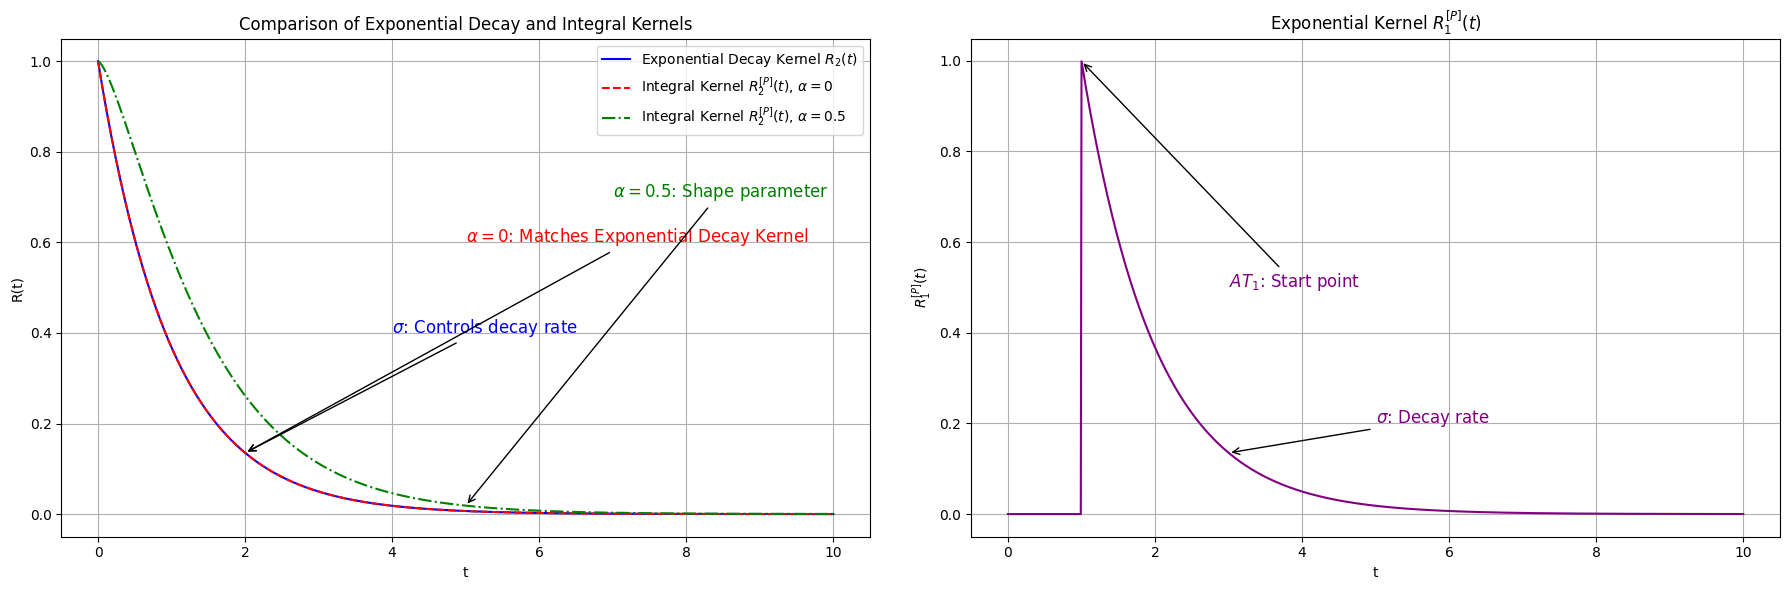
\includegraphics[width=\linewidth]{figures/method-compare.png}
            \caption{\textbf{Comparison of Kernel Functions.} 
            (Left) The plot compares the Exponential Decay Kernel \( R_2(t) \) (blue) with the Integral Kernel \( R_2^{[P]}(t) \) for two values of the shape parameter \(\alpha\): \(\alpha = 0\) (red, dashed), which matches the Exponential Decay Kernel, and \(\alpha = 0.5\) (green, dash-dotted), showing the effect of a non-zero \(\alpha\) on the kernel shape. The parameter \(\sigma\) controls the decay rate in both kernels. 
            (Right) The plot shows the Exponential Kernel \( R_1^{[P]}(t) \) (purple), which includes a shift controlled by \(AT_1\), illustrating how the start point and decay rate (\(\sigma\)) affect the kernel’s behavior.
            }
            \label{fig:comparision}
        \end{figure}
   

\end{frame}

%%% Local Variables:
%%% mode: latex
%%% TeX-master: "../topic-slide-main"
%%% End:
% method-comparision.tex
%
% Drafted by Juntang on Sept 23, 2024
%

\begin{frame}
  \frametitle{Comparison of Kernels}
        \begin{figure}
            \centering
            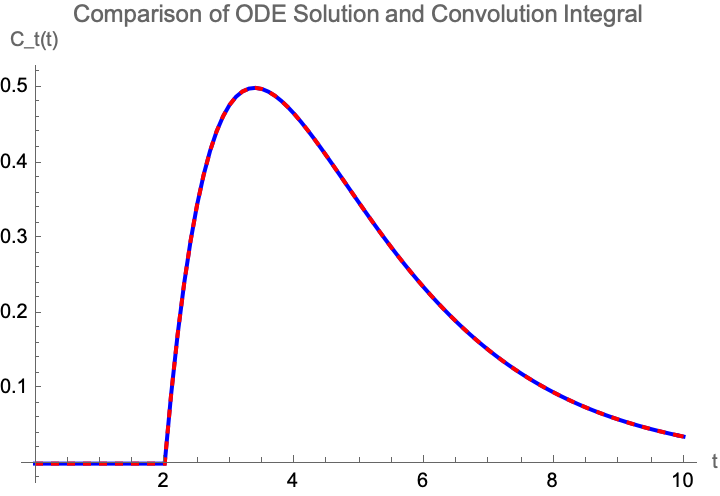
\includegraphics[width=0.6\linewidth]{figures/method-compare1.png}
            \caption{\textbf{Comparison of ODE Solution and Convolution Integral.} 
            The solid blue line represents the solution obtained from solving the ODE, while the dashed red line represents the solution computed using the convolution integral. The near-perfect overlap between the two curves confirms that the ODE solution is equivalent to the convolution of the input function with the GVF kernel.
            }
            \label{fig:comparision}
        \end{figure}
   

\end{frame}

%%% Local Variables:
%%% mode: latex
%%% TeX-master: "../topic-slide-main"
%%% End:

% \input{sections/bluered-dcp-v2}
% \input{sections/bluered-har-v2}
% \input{sections/bluered-phase}

%% ----------- Algorithm 

% %%
%% bluered-alg-formal.tex
%%


\begin{frame}{BlueRed: algorithm DT(I)}

\begin{columns}
%% double-column layout 
\begin{column}{0.45\textwidth}                 %% Left Column 

{\small \bf Descending Triangulation (I)}
% 
\begin{overprint}
\onslide<1>\scalebox{0.7}{
\begin{minipage}{1.5\textwidth}
    % !TEX root = ../digraph-main.tex

\renewcommand{\thealgocf}{}
\begin{algorithm}[H]
  \small
\SetKwInOut{Input}{Input}
\SetKwInOut{Output}{Output}
\SetKwRepeat{Do}{do}{while}
\SetKwFunction{filter}{filter}
{\bf Input:} $h$\,
// standardized clustering function with d.m. property
\\
\phantom{{\bf Input:}} $G$
//  weakly connected digraph
\\
{\bf Output:}  ${\cal B}_{\min} = ({\cal B}_{\Omega}, {\cal B}_{\theta})$  
// a pair of ordered lists
\\
{\bf Initialization:}
${\cal B}_{\Omega} \gets \{\Omega_V, \Omega_v\}, \, 
{\cal B}_{\theta} \gets \{0, \pi/4, \pi/2\}$
\\[0.1em]
\phantom{{\bf Initialization:}}
$\mbox{\rm T}  \gets \{\,\overline{\Omega_V \Omega_v}\, \}$
// candidate line-segment set

\While{\rm T $\neq \emptyset$ } {
  $ \ell = \overline{ \Omega_{a}\Omega_{b} }   \gets
  {\tt getSegment}(\, \mbox{\rm T} \,) $
  \\ 
  $\mbox{\rm T} \gets \mbox{\rm T} - \ell; \,\quad
  \gamma_{\ell} \gets -1/{\tt slope}(\,\ell\,); \,\quad
  \theta_{\ell} \gets {\rm atan}(\gamma_{\ell})$
  \\
  $ \Omega_{\ell} \gets
  \argmin\{ h(\Omega,\gamma_{\ell}) \mid \Omega \in \mathcal{L}(G) \} $ 
  \\
  \If{ $ {\tt offSegment}(\ell, \Omega_\ell) $ }
  {
    $\mbox{\rm T}_{\phantom{\theta}}\, \gets
    \mbox{\rm T} \cup
    \{ \overline{\Omega_{a}\Omega_{\ell}},  \overline{\Omega_{\ell}\Omega_{b}} \}$
    \\
    $\theta_{\rm a{\ell}} \gets 
      {\rm atan}
      \left( 
        -1 / {\tt slope}( \overline{\Omega_a \Omega_{\ell}} ) 
      \right)$ 
    \\
    $\theta_{\rm {\ell}b} \gets 
      {\rm atan}
      \left( 
        -1 / {\tt slope}( \overline{\Omega_{\ell} \Omega_b} )
      \right)$
    \\
    $ {\cal B}_{\theta}\, \gets {\tt insert}(
      {\cal B}_{\theta},
      \{ \theta_{\rm a{\ell}}, \theta_{\rm {\ell}b} \}
     ); \,\,\,
     {\cal B}_{\theta} \gets {\cal B}_{\theta}- \{\theta_{\rm \ell}\}$
    \\
    ${\cal B}_{\Omega} \gets {\tt insert}( {\cal B}_{\Omega}, \Omega_{\ell} )$
  } % End of IF 
} % End of WHILE
%
%\textcolor{red}{\em problem with updating} $\Theta$ in ${\cal B}_\min$ 
\end{algorithm}

\end{minipage}
}
\end{overprint}

\vspace*{0.5em}

{\small \bf DT(I) properties:}
  \begin{list}{$\ast$}{\itemsep = -1pt \leftmargin = 10pt}
    \footnotesize 
	\item fully autonomous, in $p$ steps
	\item theoretically guaranteed to reach ${\cal B}_{\min}$
	\item low complexity: $p\!$ $\times\!$ cost ($\gamma$-specific search)
	\item simple, efficient: successive triangulation steps
\end{list}
% 
\end{column}

\hspace*{4em}                                                          %%  make space between columns 

\begin{column}{0.42\textwidth}                                %% Right Column 
  %
  Five points: 
  \begin{enumerate}
  \item problem description, including preliminary when necessary 
  \item state of the art, citing notable  related work,
     knowledge or technology gaps 
  \item method description 
  \item analytical, experimental evidence, claims 
  \item discussion: advance made, potential promised, remaining limitation, lessons learned 
  \end{enumerate}
 %  
\end{column}
%
\end{columns}   %% End of multiple columns 
% 
\end{frame}

%%
%%
%% 

% \input{sections/bluered-alg-informal}

%% ----------- Experiments

\begin{frame}{Perfusion Analysis: Conceptual Overview}
\begin{itemize}
    \item Goal: Quantify brain tissue perfusion using Mean Transit Time (MTT)
    \item Approach: Model concentration-time curves using Gamma Variate Function (GVF)
    \item Key Assumption: Tissue response follows a gamma distribution
\end{itemize}
\end{frame}

\begin{frame}{Mathematical Framework}
\begin{align*}
    \text{GVF:} \quad C(t) &= A(t-t_0)^\alpha e^{-(t-t_0)/\beta} \\
    \text{MTT:} \quad MTT &= \alpha \beta
\end{align*}
Where:
\begin{itemize}
    \item $C(t)$: Concentration of contrast agent over time
    \item $A$: Amplitude factor
    \item $t_0$: Arrival time of contrast agent
    \item $\alpha, \beta$: Shape and scale parameters of gamma distribution
\end{itemize}
\end{frame}

\begin{frame}{Perfusion Quantification Process}
\begin{enumerate}
    \item Model tissue response: $R(t) = \frac{1}{\Gamma(\alpha)\beta^\alpha}t^{\alpha-1}e^{-t/\beta}$
    \item Assume simplified Arterial Input Function (AIF): $AIF(t) \approx \delta(t)$
    \item Tissue concentration: $C(t) = F \cdot AIF(t) \otimes R(t)$
    \item Under $\delta$-function AIF: $C(t) \approx F \cdot R(t)$
\end{enumerate}
Where $F$ is cerebral blood flow and $\otimes$ denotes convolution.
\end{frame}

\begin{frame}{Parameter Estimation}
For each voxel:
\begin{itemize}
    \item Fit GVF to observed concentration-time data
    \item Objective: Minimize error between model and observations
    \[ \min_{A,t_0,\alpha,\beta} \sum_{i=1}^{N} (C_{\text{observed}}(t_i) - C_{\text{GVF}}(t_i))^2 \]
    \item Extract MTT from fitted parameters: $MTT = \alpha \beta$
\end{itemize}
\end{frame}

\begin{frame}{Limitations and Considerations}
\begin{itemize}
    \item Simplified AIF assumption may lead to overestimation of MTT
    \item True AIF is likely also gamma-variate shaped
    \item More accurate model: $C(t) = F \cdot AIF_{\text{true}}(t) \otimes R(t)$
    \item Future work: Incorporate measured AIF for improved accuracy
\end{itemize}
\end{frame}

\begin{frame}{Results: MTT Heatmaps}
\begin{figure}
    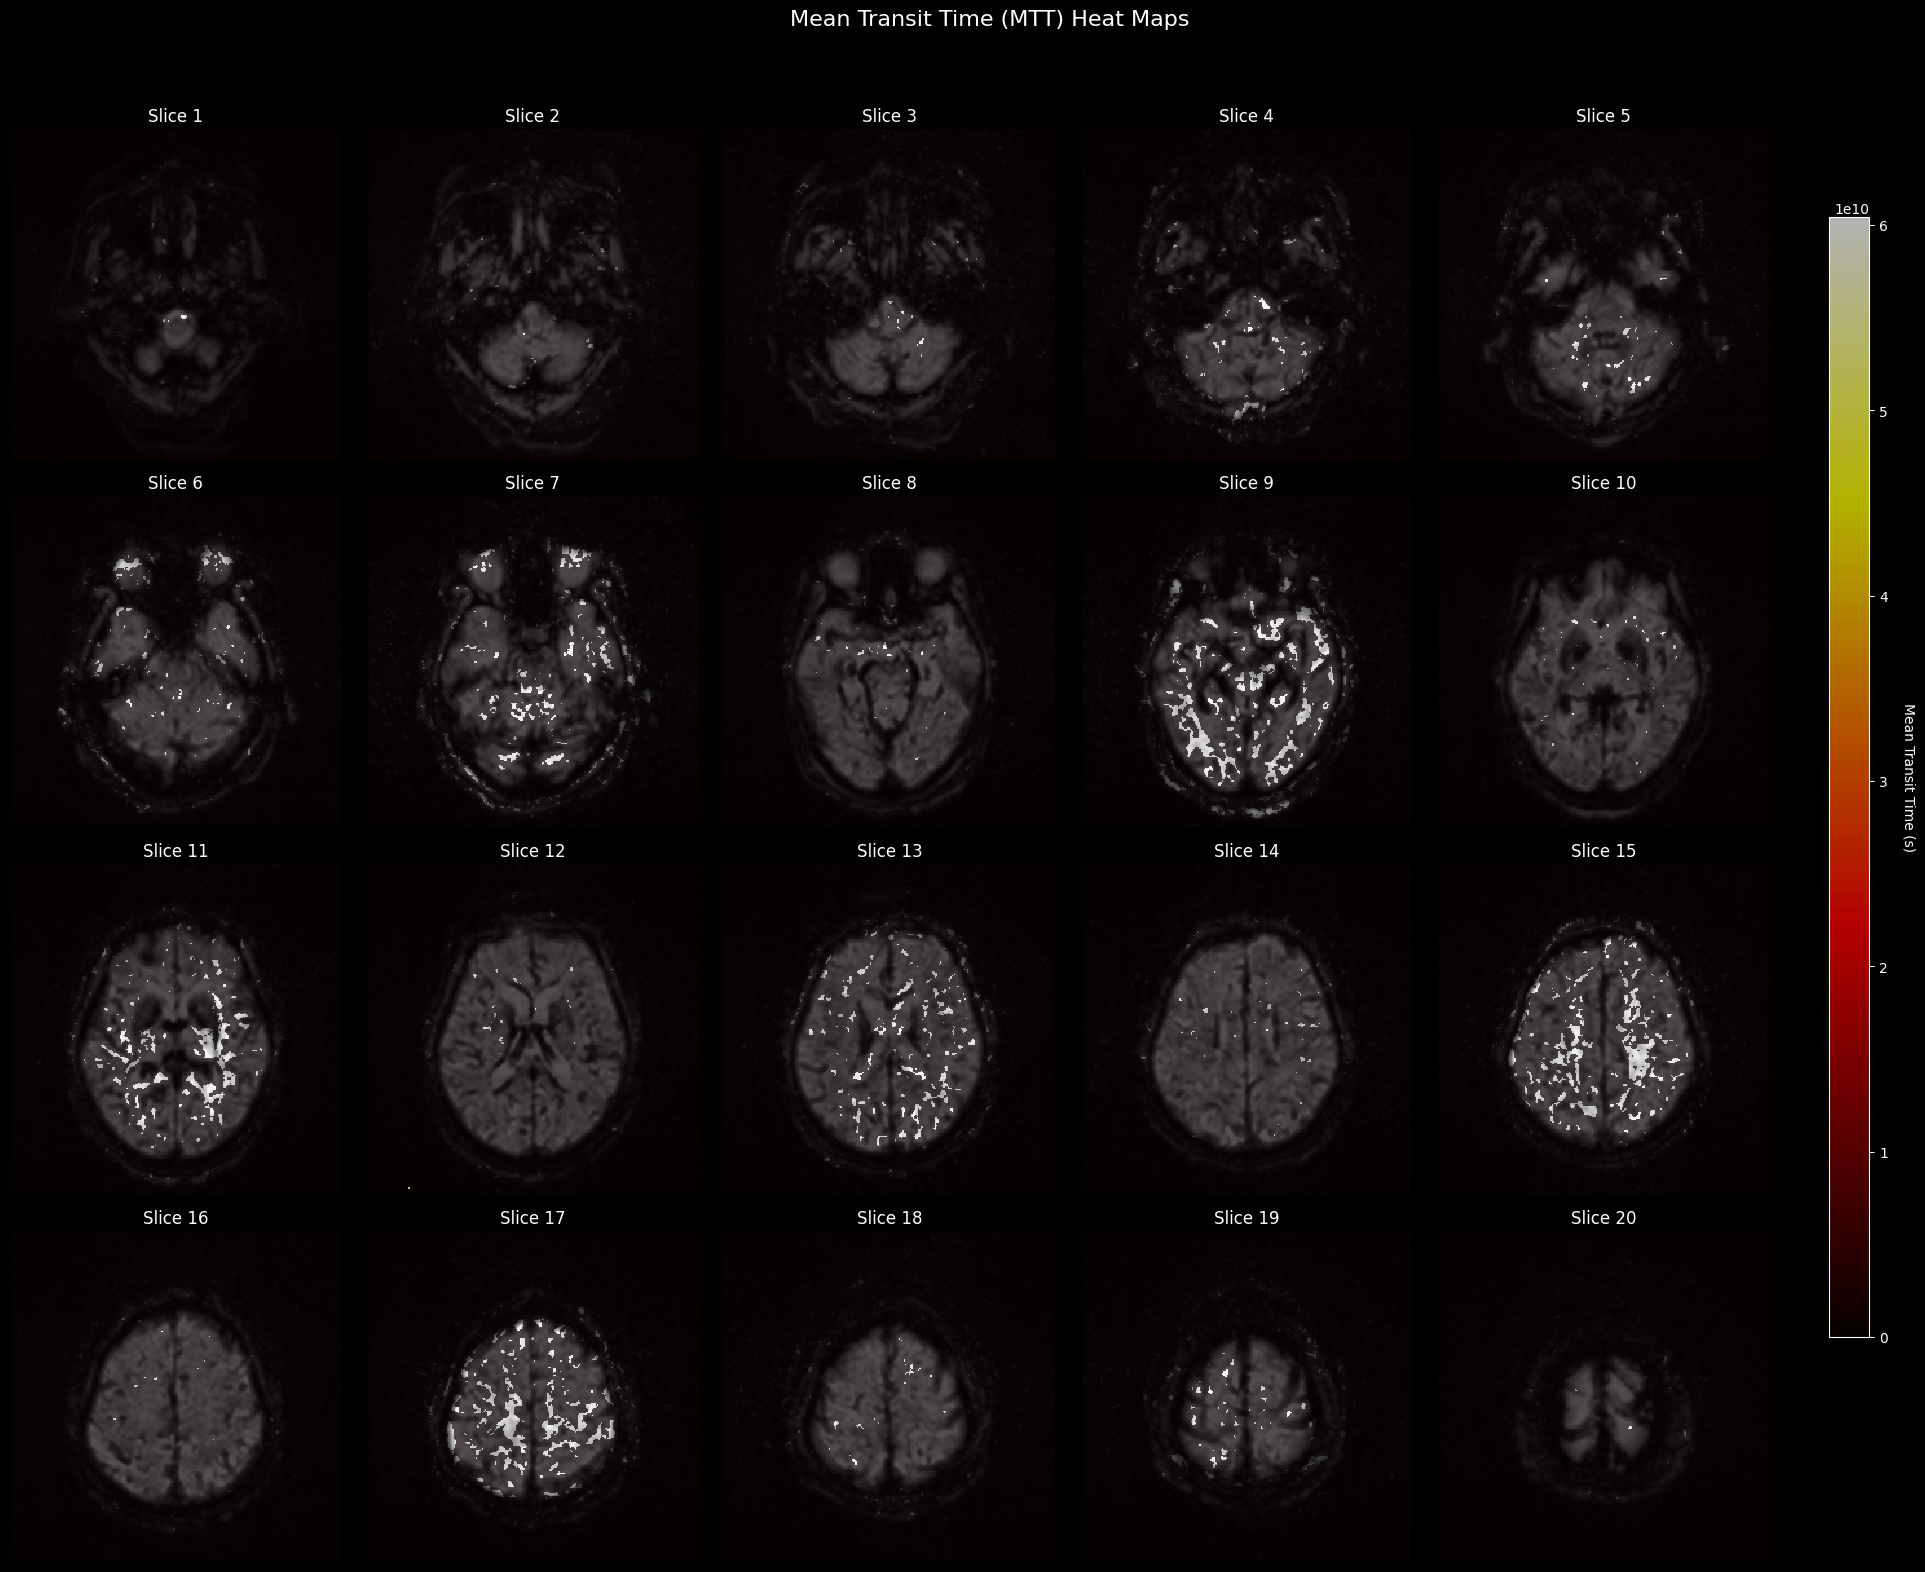
\includegraphics[width=\textwidth]{01.Oct21_GVF-MTT-HM.png}
    \caption{MTT Heatmaps overlaid on pwiMRI slices}
\end{figure}
\end{frame}

% \input{sections/exp-polblogs}
% \input{sections/exp-mnist}
% \input{sections/exp-citation}

%% ----------- Discussion

% \input{sections/discussion}


%% -----------  Acknowledgement

% !TEX root = ../digraph-main.tex

\begin{frame}{Acknowledgements}

  \begin{columns}
    \begin{column}{0.35\textwidth}
      We thank xxx for xxx 
    \end{column}
    \hspace*{2em}
    \begin{column}{0.45\textwidth}
      This work is supported in part by
      \begin{list}{$\diamond$}{\itemsep = 3pt \leftmargin=10pt}
        \item research grant xxxx
        \item research grant xxxx 
      \end{list}
    \end{column}
  \end{columns}

\end{frame}



%% ============ BIBLIOGRAPHY
\section{Bibliography}
\appendix
\begin{frame}[noframenumbering,plain,allowframebreaks]{Bibliography}
    \printbibliography[heading=none]
\end{frame}


\end{document}


%%%%

%%%%  provided by Xiaobai Sun 
%%%%
